\section{Limite inferiore per l'ordinamento per confronti}

{{[}CLRS{]} pp. 157-159}

{Fino ad ora abbiamo visto i seguenti algoritmi di ordinamento, tutti basati sul confronto.}

\begin{tabular}{|c|c|}
\hline
Algoritmo & Complessità \\
\hline
MergeSort & $\Theta(n\,log(n)))$ \\
\hline
QuickSort & Caso medio : $\Theta(n\,log(n)))$, caso pessimo : $\Theta(n^2)$ \\
\hline
HeapSort & $\Theta(n\,log(n)))$ \\
\hline
InsertionSort & $\Theta(n^2)$ \\
\hline
\end{tabular}

{Ci domandiamo, è possibile infrangere il limite inferiore di $\Theta(n\,log(n))$? Dimostreremo che NON è possibile farlo con algoritmi basati sul confronto.}

{Analizziamo il limite inferiore degli algoritmi basati sul confronto:}

{$\Omega(n)$ è il limite banale, in quanto devo analizzare n elementi. Questo limite è tuttavia irrealistico e insensato.}

{Tutti gli algoritmi basati sul confronto hanno come limite inferiore $\Omega(n\,log(n))$. Per dimostrarlo facciamo uso degli alberi di decisione.}

{Un albero di decisione è un'astrazione di un qualsiasi algoritmo di ordinamento basato sui confronti.}

\subsection{Esempio: Ordina 3 elementi}

{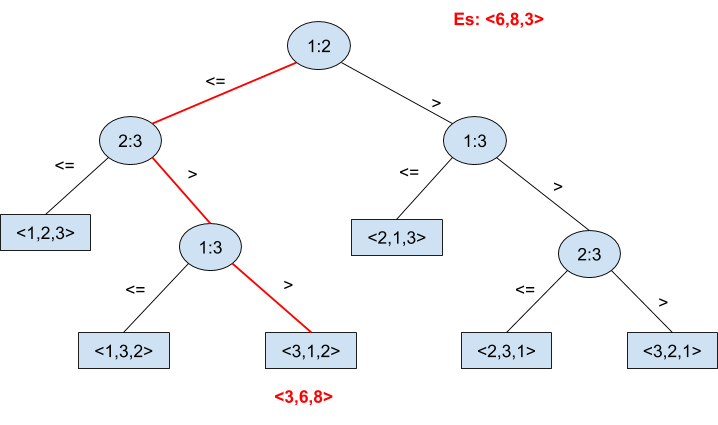
\includegraphics{images/image531.png}}

{Questa struttura assomiglia all'InsertionSort}\textsuperscript{\protect\hyperlink{cmnt15}{{[}o{]}}}

{Per un input $A = <A_1,\ldots,A_n>$ di dimensione $n$, ogni nodo interno è etichettato da una coppia $i:j$ dove $i,j$ sono indici dell'insieme da ordinare.}

\begin{itemize}
\tightlist
\item
  {$i:j$ significa confrontare $A_i$ con $A_j$}
\item
  {il sottoalbero sinistro dà i successivi confronti se $A_i \leq A_j$}
\item
  {il sottoalbero destro dà i successivi confronti se $A_i > A_j$}
\item
  {ogni foglia fornisce una permutazione dell'input tale che se io vado a prendere gli elementi dell'input, ordinati a seconda della permutazione, ottengo l'insieme ordinato in ordine crescente}
\end{itemize}

{Dato un qualsiasi algoritmo di ordinamento basato sul confronto, è possibile costruirmi gli alberi di decisione.}

\begin{itemize}
\tightlist
\item
  {Ogni valore di n è associato ad un proprio albero di decisione.}
\item
  {L'albero modella tutte le tracce possibile di esecuzione.}
\item
  {Il tempo di esecuzione (cioè il numero di confronti necessari) è la lunghezza di un cammino sull'albero.}
\item
  {Il tempo di esecuzione nel caso peggiore è il più lungo cammino dell'albero, ovvero l'altezza dell'albero.}
\end{itemize}

{Mi basta quindi trovare la dimensione dell'albero di decisione per
determinare il tempo di esecuzione.}

\subsection{Quanto è grande un albero di decisione?}

\subsubsection{Quante foglie contiene?}

{L'albero ha come minimo $n!$ foglie poichè, per essere corretto, ogni permutazione deve comparire almeno una volta.}

\paragraph{Lemma 2}

{Un albero binario di altezza h ha al più $2^h$ foglie.}

{Dimostrazione per induzione:}

\begin{itemize}
\tightlist
\item
  {Se $h=0$ abbiamo un albero costituito da un solo nodo radice che è l'unica foglia. Ovviamente con $h=0$, $1 \leq 2^h$ è verificata, infatti $1\leq 2^0$.}
\item
  {Assumiamo vera la proprietà per alberi binari di altezza $k<h$ e lo dimostro per $h$. Sia $r$ la radice dell'albero $t$. }
\end{itemize}

\begin{itemize}
\tightlist
\item
  {Se $t$ ha un solo figlio allora il numero di foglie di $t$ è uguale a quello del figlio che ha altezza $h-1$. }{Per ipotesi induttiva}{: Il numero delle foglie del sottoalbero figlio è minore di $2^{h-1}$, che è minore di $2^h$.}
\item
  {Se sono presenti entrambi il figlio sx e il figlio dx, allora il numero delle foglie è dato dalla somma delle foglie dei due sottoalberi. Siano $h_L,h_R$ le altezze dei due figli. Entrambe sono minori di $h$.}
\end{itemize}

\begin{equation}
f=f_L+f_R = 2^{h_L} + 2^{h_R} \leq 2 * 2^{max(h_L,h_R)}
\end{equation}

{$f \leq 2^{1+max(h_L,h_R)}$ ma $1+max(h_L,h_R) = h$, quindi $f \leq 2^h$}

{Quindi il numero delle foglie è compreso tra $n!$ e $2^h$.}

\paragraph{Teorema:}

{Qualsiasi algoritmo di ordinamento per confronti richiede almeno $\Omega(n\,log(n))$ confronti nel caso peggiore.}

{Dimostrazione:}

{Bisogna determinare l'altezza di un albero di decisione, dove ogni permutazione appare come foglia. Si consideri un albero di decisione di altezza $h$ con $l$ foglie che corrisponde ad un ordinamento per confronti di $n$ elementi. }

{Allora $n! \leq l \leq 2^h$ (per Lemma 2)}

{Passando al logaritmo, $h \geq log(n!)$}

{Utilizziamo l'approssimazione di \href{https://www.google.com/url?q=https://it.wikipedia.org/wiki/Approssimazione_di_Stirling\&sa=D\&ust=1523379128517000}{Stirling} per approssimare $n!$:}

\begin{equation}
n! \simeq \sqrt{2\pi n }* {(\frac{n}{e})}^n
\end{equation}

{Per n sufficientemente grande, considero solo il termine più grande}

$h \geq log({(\frac{n}{e})}^n)$

{Per proprietà dei logaritmi}

$h \geq n*log(\frac{n}{e})$

{$h \geq n*(log(n) - log(e))$ , il secondo algoritmo è costante}

$n \geq n * log(n)$

{Non ci può essere quindi un algoritmo basato sui confronti minore di $n * log(n)$}

\paragraph{Corollario:}

{Gli algoritmi HeapSort e MergeSort sono algoritmi di ordinamento per confronti asintoticamente ottimali.}

{Dimostrazione:}

{I limiti superiori dei sue algoritmi sono $O(n\,log(n))$ nei tempi di esecuzione corrispondono al limite inferiore $\Omega(n\,log(n))$ nel caso peggiore dato dal teorema.}

{Se elimino il modello basato sui confronti, posso battere il limite inferiore di $\Omega(n\,log(n))$? SI.}
